% Masterthesis
%
% Multiscale Modelling Group of Jun.-Prof. Birgit Strodel
%
% Author:
% Oliver Schillinger

 

\ifdefined\isdraft
    \documentclass[english, a4paper, 12pt, titlepage, draft]{article}
\else
    \documentclass[english, a4paper, 12pt, titlepage, final]{article}
\fi
 

\usepackage{geometry}
\usepackage[british]{babel}
\usepackage{graphicx,hyperref,url,color,cite}
\usepackage[table]{xcolor}
\usepackage{mathtools}
\usepackage[latin1]{inputenc}

\definecolor{fzjblue50}{cmyk}{1,0.2,0.05,0.50}
\definecolor{fzjblue35}{cmyk}{1,0.2,0.05,0.35}
\definecolor{fzjblue30}{cmyk}{1,0.2,0.05,0.30}
\definecolor{fzjblue20}{cmyk}{1,0.2,0.05,0.20}
\definecolor{fzjblue10}{cmyk}{1,0.2,0.05,0.10}
\definecolor{fzjgray80}{cmyk}{0,0,0,0.8}
\definecolor{fzjgray50}{cmyk}{0,0,0,0.5}
\definecolor{fzjgray30}{cmyk}{0,0,0,0.3}

\usepackage{framed}
\definecolor{shadecolor}{cmyk}{1,0.2,0.05,0.10}

\usepackage{mdframed}
\mdfsetup{
    framemethod=tikz,
    linewidth=10pt,
    linecolor=fzjblue50,
%    innerlinewidth=10pt,
%    middlelinewidth=10pt,
%    outerlinewidth=10pt,
%    innerlinecolor=red,
%    middlelinecolor=green,
%    outerlinecolor=blue,
    backgroundcolor=fzjgray30,
    roundcorner=15pt}
%\newmdenv[linecolor=black,backgroundcolor=fzjblue10,roundcorner=10pt,linewidth=5pt]{titlebox}
%\newmdenv[linecolor=red]{titlebox}

\usepackage{setspace}
\usepackage[version=3]{mhchem}

\hypersetup{
    %bookmarks=false,                      % show bookmarks bar?
    unicode=true,                          % non-Latin characters in Acrobat’s bookmarks
    pdftoolbar=true,                       % show Acrobat’s toolbar?
    pdfmenubar=true,                       % show Acrobat’s menu?
    pdffitwindow=false,                    % window fit to page when opened
    pdfstartview={FitH},                   % fits the width of the page to the window
    pdftitle={Masterthesis},               % title
    pdfauthor={Oliver Schillinger},
    pdfsubject={Masterthesis},             % subject of the document
    pdfcreator={Oliver Schillinger},       % creator of the document
    pdfproducer={Oliver Schillinger},      % producer of the document
    pdfkeywords={Lipase} {CitA} {GROMACS}, % list of keywords
    pdfnewwindow=true,                     % links in new window
    colorlinks=true,                       % false: boxed links; true: colored links
    linkcolor=black,                       % color of internal links
    citecolor=blue,                        % color of links to bibliography
    filecolor=red,                         % color of file links
    urlcolor=cyan                          % color of external links
}

\newcommand{\PDB}[1]{\href{http://pdb.rcsb.org/pdb/explore/explore.do?structureId=#1}{#1}}

% Formula typesetting commands
\newcommand{\vect}[1]{\mathbf{#1}}
\newcommand{\norm}[1]{\left\Vert#1\right\Vert}
\newcommand{\fun}[2]{#1\left(#2\right)} 
\newcommand{\vfun}[2]{\vect{#1}\left(#2\right)} 
\newcommand{\vfunv}[2]{\vect{#1}\left(\vect{#2}\right)} 

% Figure template
%\begin{figure}
%    \centering
%    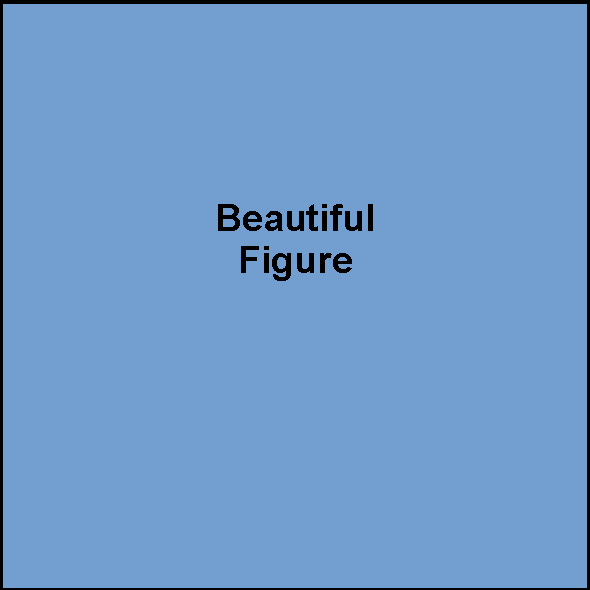
\includegraphics[width=0.5\textwidth]{figures/draft/draft.pdf}
%    \caption{}
%    \label{fig:}
%\end{figure} 


% ============================================================================ %


\begin{document}

% ============================================================================ %

\onehalfspacing

\section{Methods}
\subsection{Molecular Dynamics}
\subsubsection{Integrators}

\subsubsection{Force Fields}
\label{sec:forcefields}

An exact calculation of the behaviour of a molecular system involves solving the Schr\"odinger equation for all electrons and nuclei.
As the computaional complexity for this problem grows extremely fast with increasing system size, the direct solution of all but the smallest molecular system is infeasible.
Parameterized, analytical descriptions have been developed for a simplified description of interatomic interactions in and between molecules that enable simulations of large molecular systems.
The mathematical form of these equations is inspired by knowledge of the physics and chemistry that govern molecular interactions.
The parameters are chosen to reproduce energy functions of quantum mechanical descriptions of model systems.
As the large number of parameters, the choice of the model systems and the quantum chemical methods used for reference computations are all degrees of freedom in the paremterization, several different sets of parameters exist.
A set of equations with its corresponding parameters is called a force field.
This section first discusses the mathematical form of relatively simple, non polarizable force fields and then gives reasons for the choice of a particular implementation.

\paragraph{Lennard-Jones Potential}
A simple but often reasonable model of atomic structure treats atoms as nuclei surrounded by a diffuse electron cloud.
Some elements possess a permanent dipole moment due to the shape and occupation of their electronic orbitals.
Three kind of interactions between electron clouds give rise to the Van-der-Waals interaction, which is one contribution to the Lennard-Jones potential.
First, two permanent dipoles interact and will attract or repel each other depending on their mutual alignment.
The second contribution to the Van-der-Waals interaction comes from dipoles induced in the electron cloud by permanent dipoles of neighbouring atoms.
This interaction is attractive, as the induced dipole will have the same polarization as the inducing dipole due to repelling electron clouds.
Finally, the electron clouds of two unpolarized atoms repel each other, therefore inducing dipoles that in turn give rise to a dipole--dipole interaction.
The sum of these 3 effects is the source of the Van-der-Waals interaction and gives rise to an overall attractive force that decays with the sixth square root of the inter atomic distance.

Two atoms that approach each other will be affected by the Pauli exclusion principle that prohibits electrons from having the same state.
This prevents two atoms to occupy the same space and will result in a repelling force at close distances.
This and the dipole interactions of the electron clouds together are cast in the Lennard Jones potential that contains a term for short range repulsion and one for long range attraction (Figure \ref{fig:LJ} and equation \ref{eq:LJ}).
For each pair of elements a force field needs to specify two parameters to define their equilibrium distance and the depth of the interaction well.
Many force fields list only one set of parameters per element and give a relation for the computation of parameters for the Lennard-Jones interaction of two different elements.
The Lennard-Jones interaction converges fast to a constant value, and with it the resulting force goes to zero.
This fast convergence makes a truncation at a suitable cutoff distance possible.
However, for an accurate computation of the potential energy, the constant term at this cutoff distance needs to be accounted for.

\begin{figure}
    \begin{minipage}[]{0.45\linewidth}
        \centering
        \vfill
        \begin{equation}
            V_{LJ}(r_{ij}) = \frac{C^{(12)}_{ij}}{r^{12}_{ij}} - \frac{C^{(6)}_{ij}}{r^{6}_{ij}}
            \label{eq:LJ}
        \end{equation} 
        \vfill 
    \end{minipage}
\hspace{0.5cm}
    \begin{minipage}[]{0.45\linewidth}
        \centering
        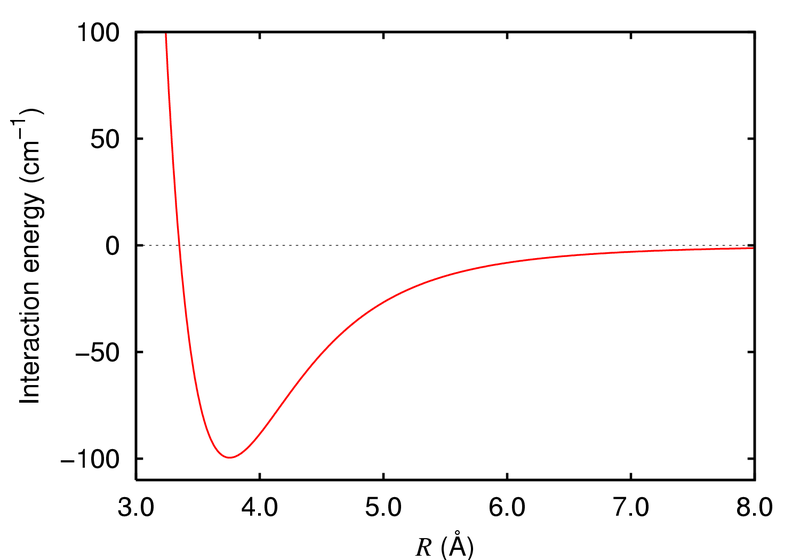
\includegraphics[width=\textwidth]{figures/Argon_dimer_potential.png} 
    \end{minipage}
    \caption{Left: Lennard-Jones potential formula ($C^{*}_{ij}$ are the coefficients to be parameterized and $r_{ij}$ is the inter atomic distance). Right: Argon dimer potential. Source: \url{http://en.wikipedia.org/wiki/File:Argon_dimer_potential.png}}
\label{fig:LJ}
\end{figure}


\paragraph{Coulomb potential}
The computation of the coulomb interaction (equation \ref{eq:CoulombPot}, $q_i$ is the charge on atom $i$ and $\epsilon_0$ is the dielectric constant of vacuum) is particularly tricky as the electrostatic force decays slowly with increasing distance and suffers from ill convergence.
This problem is treated with sophisticated methods for long range electrostatic interactions as described in section \ref{sec:PME}.
The partial charges on each atom that are needed for the evaluation of the coulomb potential are also part of the force field parameter set and are usually derived from quantum chemical calculations.

\begin{equation}
    V_C(r_{ij}) = \frac{1}{4\pi \epsilon_0} \frac{q_i q_j}{r_{ij}}
    \label{eq:CoulombPot}
\end{equation}

\paragraph{Bonded Forces}
Apart from the non-bonded inter atomic forces there also exist interaction potentials due to bonds between the atoms of a molecule.
Bond stretching (equation \ref{eq:bonded}), bond angle bending (equation \ref{eq:angle}), proper and improper dihedral angles (equations \ref{eq:dihedral} and \ref{eq:improper} respectively) can all be modelled by harmonic potentials, but more sophisticated mathematical forms exist as well.
Bond stretching is defined by an equilibrium distance between two atom types $r^0_{ij}$ and an interaction constant $k^b_{ij}$.
Bond angles are parameterized by an equilibrium angle between three atom types and a constant ($\theta^0_{ijk}$, $k^a_{ijk}$).
Dihedral and improper dihedral angles depend on interaction constants and equilibrium angles between planes spanned by three atoms $ijk$ and $jkl$ ($\phi^0_{ijkl}$, $\xi^0_{ijkl}$, $k^d_{ijkl}$ and $k^{id}_{ijkl}$).


\begin{eqnarray}
    V_b(r_{ij})        & = & \frac{1}{2} k^b_{ij}(r_{ij}-r^0_{ij})^2 \label{eq:bonded} \\
    V_a(\theta_{ijk})  & = & \frac{1}{2} k^a_{ijk}(\theta_{ijk}-\theta^0_{ijk})^2 \label{eq:angle} \\
    V_d(\phi_{ijkl})   & = & k^d_{ijkl}(1+cos(n\phi_{ijkl}-\phi^0_{ijkl})) \label{eq:dihedral}\\
    V_{id}(\xi_{ijkl}) & = & \frac{1}{2} k^{id}_{ijkl}(\xi_{ijkl}-\xi^0_{ijkl})^2 \label{eq:improper}
\end{eqnarray}




The described potentials are only the simplest to use in molecular force fields ant a variety of others exist that result in more accurate representations, especially for the dihedral angles.
A great variety of force fields exists and a careful and well informed choice about the set of equations and parameters that can model the system under investigation best has to be made.
Recent benchmarks of protein force fields give insights into the strengths and weaknesses of the available options \cite{proteinFF}, indicating that one of the most up to date corrections to the widely used amber force field (\texttt{amber99sb-ildn-nmr}) \cite{amber99sb-ildn-nmr} is the best choice for simulations of proteins in explicit solvent.
For the cited benchmark a statistical evaluation of the performance of various force fields compared to real experiments was performed.
A number of di- and tripeptides served as model systems for chemical shift measurements in NMR experiments.
The deviations of the measurements from chemical shifts, computed on the basis of molecular dynamics trajectories performed with the investigated force fields, are reported.
In general, older force field parameterization sets performed worse than newer corrections for all force fields studied.
The chosen correction to the \texttt{amber99} force field performed best in simulations of ubiquitin, the only full length protein studied in the benchmark.
This led to the decision to use this force field for the reported experiments.

% ==================================== %

\subsubsection{Citrate Parameterization}

The \texttt{amber99sb-ildn-nmr} force field parameterizes only amino and nucleic acids, biologically relevant ions, water and a very limited set of other molecules.
It does not include parameters for citrate.
Force field parameters for use with the amber force fields were generated with the tool ACPYPE \cite{ACPYPE}.
ACPYPE acts as an interface to the Antechamber programs from the Ambertools package \cite{antechamber}.
In particular, it uses the general amber force field (GAFF) \cite{GAFF} to generate topologies for small organic molecules that can directly be used with GROMACS in combination with one of the amber force fields.
GAFF is an empirical approach to force field parameterization for arbitrary molecules.
It inherits the Van-der-Waals parameters from the \texttt{amber99} force fields directly.
Parameters for the bonded interactions have been fitted to \textit{ab initio} calculations and equilibrium bond length and angles have also been estimated by real experiments.
A crucial point in topology generation with GAFF is the assignment of partial charges.
Ideally, this should be done based on elaborate quantum chemical calculations.
There exist however other means of empirical partial charge assignments.
The charges assigned to citrate for this research have been estimated with the AM1-BCC model \cite{am1bcc_method} \cite{am1bcc_validation}.
This model tries to generate charges that emulate the electrostatic potential of \textit{ab initio} Hartree Fock calculations with the HF/6-31G* basis set.


% ==================================== %

\subsubsection{Long--Range Electrostatics}
\label{sec:PME}

The electrostatic potential decays relatively slowly with increasing distance (equation \ref{eq:CoulombPot}).
As a result, the computation of electrostatic interactions converges slowly and cannot simply be cut off at a specified distance without introducing significant artifacts \cite{FrenkelSmit}.
Efficient techniques have been developed to arrive at and accurate and, at the same time, fast computation of the electrostatic energy in periodic systems.
The problem to be solved is the estimation of a solution to Poisson's equation:

\begin{equation}
    -\nabla^2 \phi(\vect{r}) = 4 \pi \rho(\vect{r}),
\end{equation}

where $\phi$ is the electrostatic potential and $\rho$ is the charge density function.
Gaussian units are used.

All approaches to tackle long range electrostatics efficiently rely either on multipole expansions or on summations in reciprocal space that converge much faster than the corresponding sums in direct space.
The starting point is to split the electrostatic interaction into an easily computable short range and a harder to estimate long range part:

\begin{equation}
    \phi(\vect{r}) = \phi_{sr}(\vect{r}) + \phi_{lr}(\vect{r})
\end{equation}

The short range part is evaluated directly by a sum over all atoms up to the short range cutoff distance.
The long range part is then computed in reciprocal space by Fourier transforming the charge distribution, performing the evaluation of the fast converging reciprocal electrostatic interaction function and back transforming the result to direct space.
The straight forward implementation of this is known as Ewald summation, invented by P.P. Ewald in 1921 \cite{Ewald}.
The Ewald method has a complexity of $\mathcal{O}(n^{3/2})$ and scales therefore only to limited system sizes.

A method that scales a lot better, at the order of $\mathcal{O}(n \cdot log(n))$, is the Particle-Mesh-Ewald method (PME) \cite{PME}.
Instead of Fourier transforming the long range part of the electrostatic interaction directly, the charges are assigned to the nodes of a grid covering the direct space.
The grid can then be transformed to reciprocal space utilizing the fast Fourier transform algorithm (FFT), which itself scales as $\mathcal{O}(n \cdot log(n))$.
After evaluation of the interaction in reciprocal space, the inverse FFT transforms the result back to direct space.
This techniques enables efficient treatment of long range interactions that scales well to large system sizes.
In the GROMACS MD package, the FFT is done in parallel on a designated number of processors to limit communication to a minimum.



% ==================================== %

\subsubsection{Temperature \& Pressure Control}
\label{sec:tempPressControl}

According to the ergodic hypothesis, a histogram of states visited by a thermodynamical system during an infinite time span equals a histogram of an infinite number of copies of the same system in thermodynamical equilibrium at one instant of time.
In other words, averages of system properties over time will equal averages over states in phase space.
These distributions of states at thermodynamic equilibrium are summarized in the concept of ensembles \cite{Atkins}. 
Each of a number of possible ensembles (i.e. distributions of states) is associated with system properties that are constant for all states of that ensemble.
The thermodynamic ensemble that is produced by a molecular dynamics simulation is controlled by the macroscopic properties that are kept constant during the simulation
The ensemble directly affects the behaviour of the system and therefore the measured quantities.
A naive approach to molecular simulation would keep the number of particles ($N$), the system volume ($V$) and the total energy of the system ($E$) constant, as this does not require any control of extensive, and thus hard to influence quantities.
This will yield distributions from the microcanonical, or $NVE$ ensemble, which does not correspond to any situation that is easy to create in a laboratory.
Two other ensembles result in distributions that are much more directly comparable to real world experiment.
The canonical, or $NVT$ ensemble, requires a proper control of temperature (T) and reflects experimental conditions of constant volume and constant temperature.
The grand canonical ensemble, or $NPT$ ensemble, needs an additional mechanism to control the pressure (P).
$NPT$ is the desired ensemble for most biomolecular simulations, as it corresponds directly to \textit{in vivo} situations, where the pressure and temperature are controlled by the environment and in general thought to remain constant on chemically relevant time scales.

Several algorithms exist for pressure control during MD simulations.
The Berendsen algorithm (\cite{BerendsenTempControl}) rescales the velocities in order to match the differential equation

\begin{equation}
    \frac{dT}{dt} = \frac{T_0 - T}{\tau},
\end{equation}

that couples the system exponentially with a time constant $\tau$ to a heat bath of temperature $T_0$.
The Berendsen thermostat suppresses fluctuations of kinetic energy and therefore does not generate a proper thermodynamic ensemble. It might still be used for equilibration purposes.

The Nose-Hoover thermostat (\cite{Nose}, \cite{Hoover}) extends the system Hamiltonian by coupling to a thermal reservoir with a friction term $\xi$.
The reservoir has its own momentum $p_{\xi}$, a mass-like parameter $Q$ and follows its own dynamic equations of motion:

\begin{equation}
    \frac{dp_{\xi}}{dt} = (T-T_0),
\end{equation}

coupling the reservoir momentum to a reference temperature $T_0$.
The new equation of motion for the particles is:

\begin{equation}
    \frac{d^2\vect{r}_i}{dt^2} = \frac{\vect{F}_i}{m_i} - \frac{p_{\xi}}{Q} \frac{d\vect{r}_i}{dt}
\end{equation}

The Nose-Hoover thermostat can be extended to couple the heat reservoir to another bath, which in turn couples to a further bath and so forth to generate a chain of baths.
This Nose-Hoover chain is guaranteed to be ergodic in the limit of infinite chain length.
The system temperature under control of a Nose-Hoover chain will oscillate around a reference value and it is therefore not suited for equilibration if the system starts out at a totally different temperature.

A third temperature control algorithm is the velocity rescaling thermostat, which, as the name suggests, rescales the velocities similar to the Berendsen thermostat with the improvement of an additional stochastic term that ensures the generation of a proper thermodynamic ensemble distribution.

Pressure control happens along the same lines of the algorithms outlined for temperature control.
A Berendsen analog for pressure coupling exists and the Parinello-Rahman (\cite{ParrinelloRahman}) and Martyna-Tuckerman-Tobias-Klein (MTTK, \cite{MTTK}) algorithms are similar in spirit to the Nose-Hoover thermostat, coupling the pressure to a pressure bath.
One additional complication of pressure control is the definition and computation of the pressure in a bulk system.
It is defined with the virial equation:

\begin{equation}
    PV = Nk_BT + \frac{1}{D} \left< \sum^N_{i=1}\vect{r}_i \vect{F}_i \right>
\end{equation}

The virial equation relates the pressure to the average over the forces acting on all particles.
The pressure computed in this way is a highly fluctuating quantity and only its average can be meaningfully interpreted.

% ==================================== %

\subsubsection{Water Model}

Despite being a small and at first sight simple molecule, the properties of water are particularly hard to model properly.
This is mainly due to the complex interactions between water molecules that form complicated networks, especially in the liquid phase.
A wide range of models have been invented, some of which get close to reality in the prediction of water properties like density, dipole moment, dielectric constant and the self diffusion, but none of them can be regarded as perfect as each has its own shortcomings.
A detailed overview of water models is given at \url{http://www.lsbu.ac.uk/water/models.html}.
Water models can be distinguished by the geometry that they adapt to model real water.
Planar models exist that either place all partial charges on the atoms themselves (e.g. SPC and tip3p water models), or introduce a virtual interaction site on which a partial charge is deposited (e.g. tip4p water model).
This latter was introduced to improve the prediction of the dipole moment.
More elaborate models are of tetrahedral shape with partial charges pointing in the direction of the oxygen lone pairs (e.g. tip5p water model).
Despite their larger complexity, these models do not necessarily perform better in molecular dynamics simulations.
Also, for the computational treatment of different systems, different water models might be optimal.
Based on the force field benchmark reported in \cite{proteinFF}, the force field used in this study (\texttt{amber99sb-ildn-nmr}) performs best in combination with the tip4p-ew water model.
Therefore this combination was used for the reported simulations.






\subsection{GMIN}

Several Basin Hopping runs have been performed with GMIN to find energy minima of the fusion protein.
Long runs were set up for higher accuracy and short runs for fast result availability.
Most parameters were common to all runs.
Chirality checks were switched off, so were checks for the cis/trans isomerisation of the peptide bond.
The temperature for the Monte Carlo moves was set to 298 K.
The sloppy and tight conversion criteria for the root mean square (RMS) force during the energy minimizations were set to 0.01 and 0.02 kcal/mol/nm respectively.
The acceptance ratio of Monte Carlo moves was specified to be 0.3.
Energy minima had to have at least an energy difference of 1.0 kcal/mol to be considered as different energy basins.
All runs were performed with the CHARMM22 all-atom protein force field \cite{CHARMM22} together with the implicit solvent model FACTS \cite{FACTS}.
For FACTS, the solute dielectric constant was set to $\epsilon = 1.0$ and the nonpolar surface tension coefficient to $\gamma$ = 0.015 kcal/(mol $\cdot$ A$^2$).
Only dihedral angle Monte Carlo moves have been performed for the $\phi$ and $\psi$ backbone dihedral angles in the linker domain between the two proteins.
During the energy minimization, all atoms were allowed to move, resulting in different side chain conformations for the output structures.

Several simulations have been run with increasing number of Basin Hopping steps in the sequence 100, 500, 1000, 5000 and 10000.
Apart from that, three runs with 1000 Basin Hopping steps each and different values for the sloppy convergence criterium during energy minimization were performed: 0.05, 0.1 and 0.5 kcal/mol RMS force.
In addition 40 energy basin structure from previous research have been acquired.
Of each Basin Hopping run the 10 structures with minimal energies were kept for subsequent analysis.
The Basin Hopping simulations thus resulted in a total of 120 structures.



% ============================================================================ %

\section{Results}

\subsection{Uncomplexed CitAP MD}

To arrive at a quantitative description of the CitAP binding pocket geometry, two distances have been defined (Figure \ref{fig:CitA_pocket}).
Leucine 102 occupies the turning point of the minor loop.
Its backbone nitrogen atom forms a hydrogen bond with the citrate molecule when the pocket is in its closed conformation.
Glutamic acid 74 is located opposite to Leucine 102 in the binding pocket and Tyrosine 56 at the bottom of the acitve site.
From a visual inspection of the open and closed conformations it is apparent that the distances between the backbone nitrogen of Leucine 102 and the \ce{C_{$\alpha$}} atoms of Glutamic acid 74 and Tyrosine 56 give a good geometrical description, as these are minimal in the closed and maximal in the open conformation.
The crystal structure distances of the LEU102:N to TYR56:C$_{\alpha}$ and LEU102:N to GLU74:C$_{\alpha}$ are 9.3 and 9.9 \r{A}ngstrom respectively.

The results of 100 ns molecular dynamics simulations of CitAP with and without a bound citrate molecule are shown in Figure \ref{fig:CitA_opening_distances}.
The starting structure for both simulations was the citrate bound crystal structure except for the citrate molecule.
While the citrate free pocket opens up within nanoseconds and stays in the open conformation for the entire course of the simulation, the citrate interactions in the bound form keep the minor loop tightly closed, covering citrate in the binding pocket.
For the first half of the simulation, the LEU102:N to GLU74:C$_{\alpha}$ distance gets even smaller than the crystal structure reference distance.
This is likely due to intense hydrogen bonding with the citrate ligand and the absence of crystal packing artifacts in solution.
After approximately 50 ns, the two distances cross in Figure \ref{fig:CitA_opening_distances}, meaning that the LEU102:N to TYR56:C$_{\alpha}$ distance now gets slightly longer than before and the LEU102:N to GLU74:C$_{\alpha}$ slightly shorter.
These two situation in the first and in the second half of the 100 ns trajectory likely correspond to two local minima of the closed state of CitAP.


\begin{figure}
    \centering
    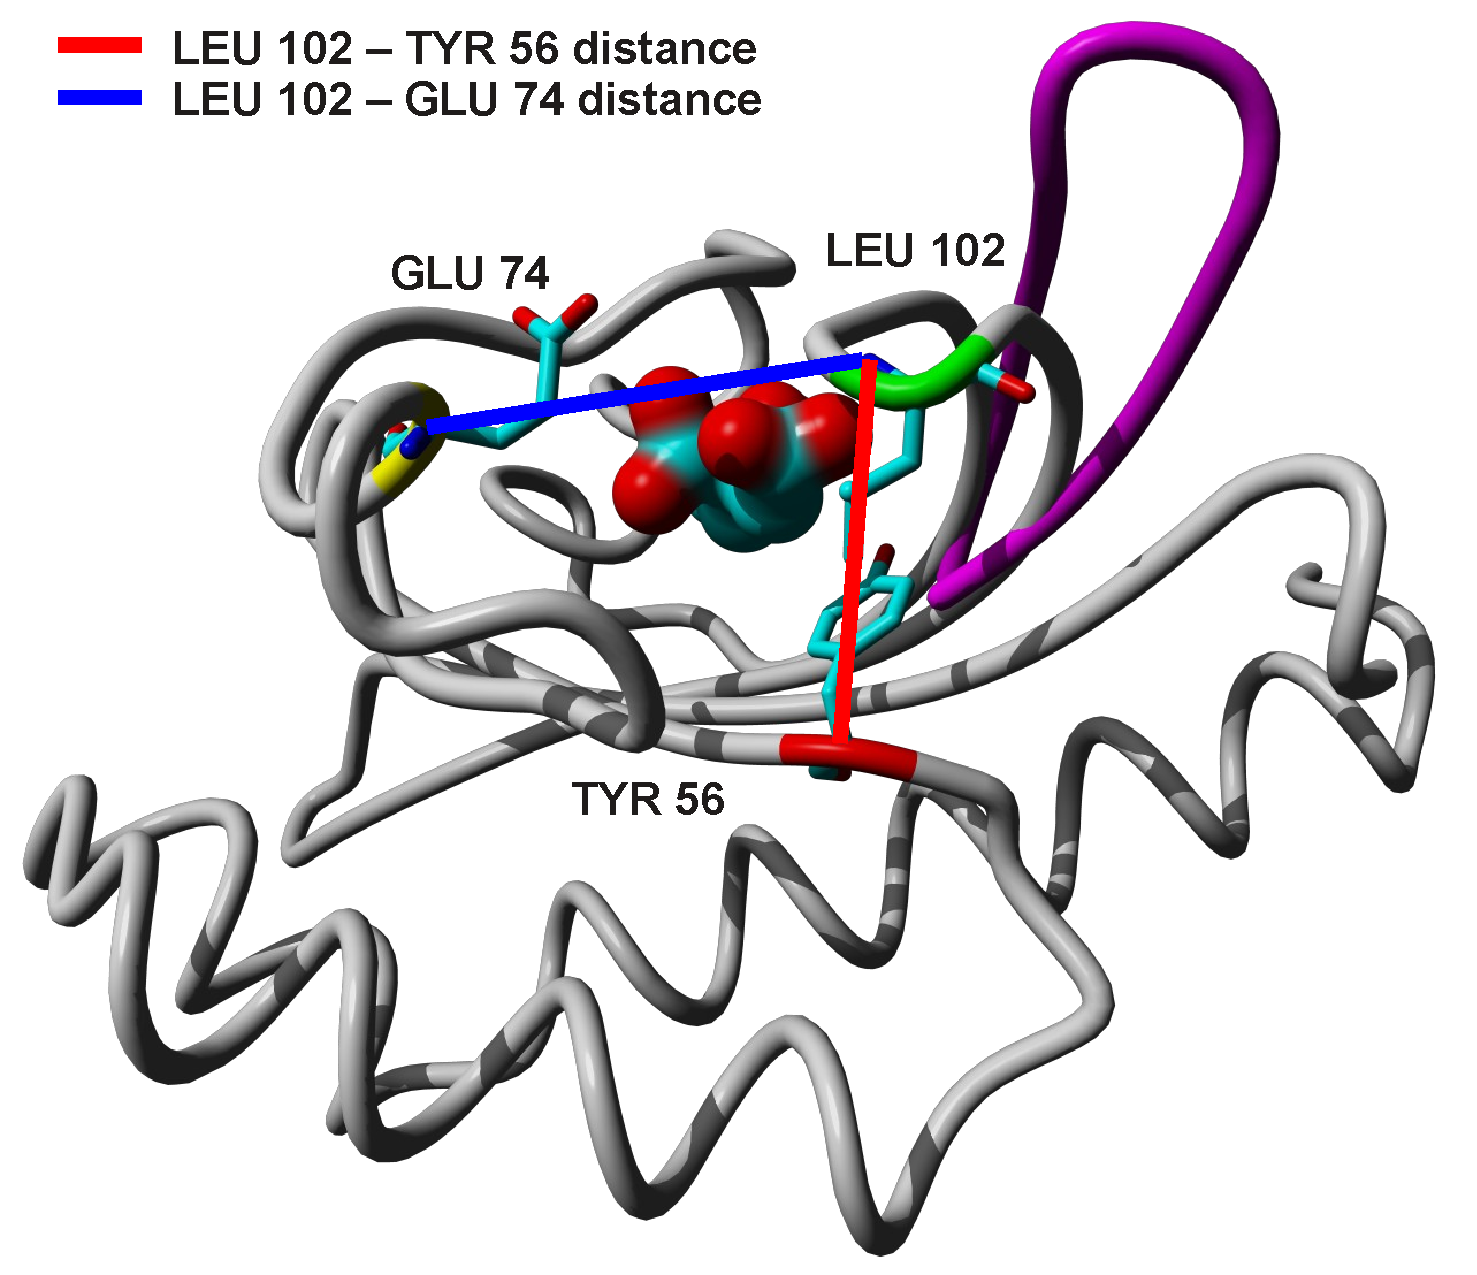
\includegraphics[width=0.7\textwidth]{figures/CitA_pocket2.pdf}
    \caption{To measure the geometry of the CitAP binding pocket, two distances were introduced: The distance between the backbone nitrogen of Leucine 102 and the \ce{C_{$\alpha$}} atoms of Glutamic acid 74 (blue) and Tyrosine 56 (red).
    The purple loop shows the minor loop in the fully extended open conformation.}
    \label{fig:CitA_pocket}
\end{figure}        

\begin{figure}
    \centering
    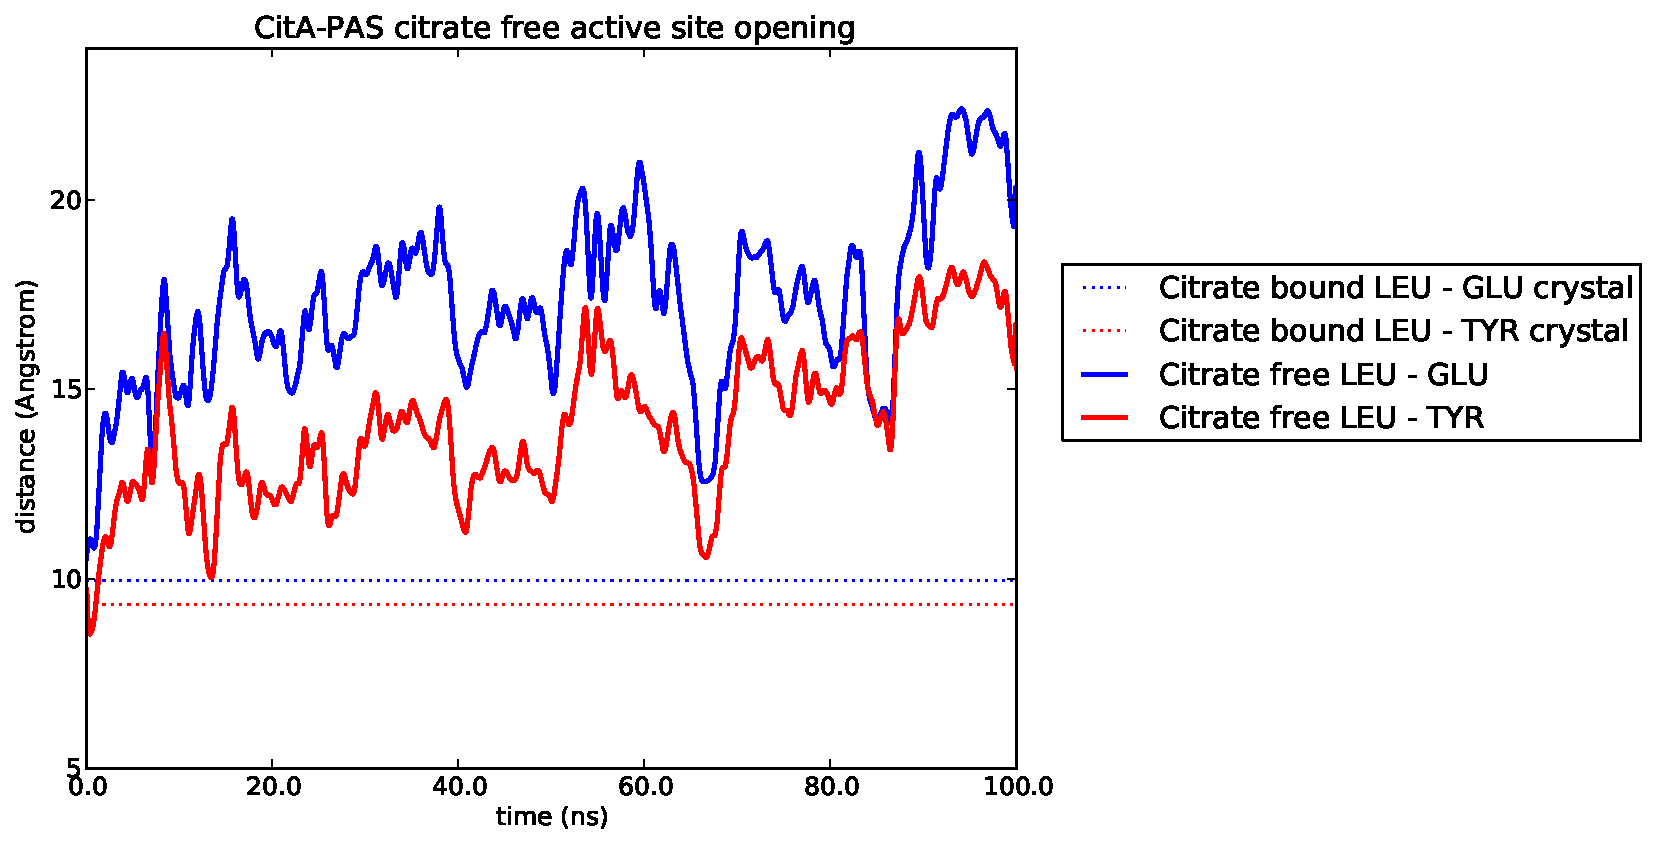
\includegraphics[width=1.0\textwidth]{figures/CitA_opening_citrate_free.pdf}
    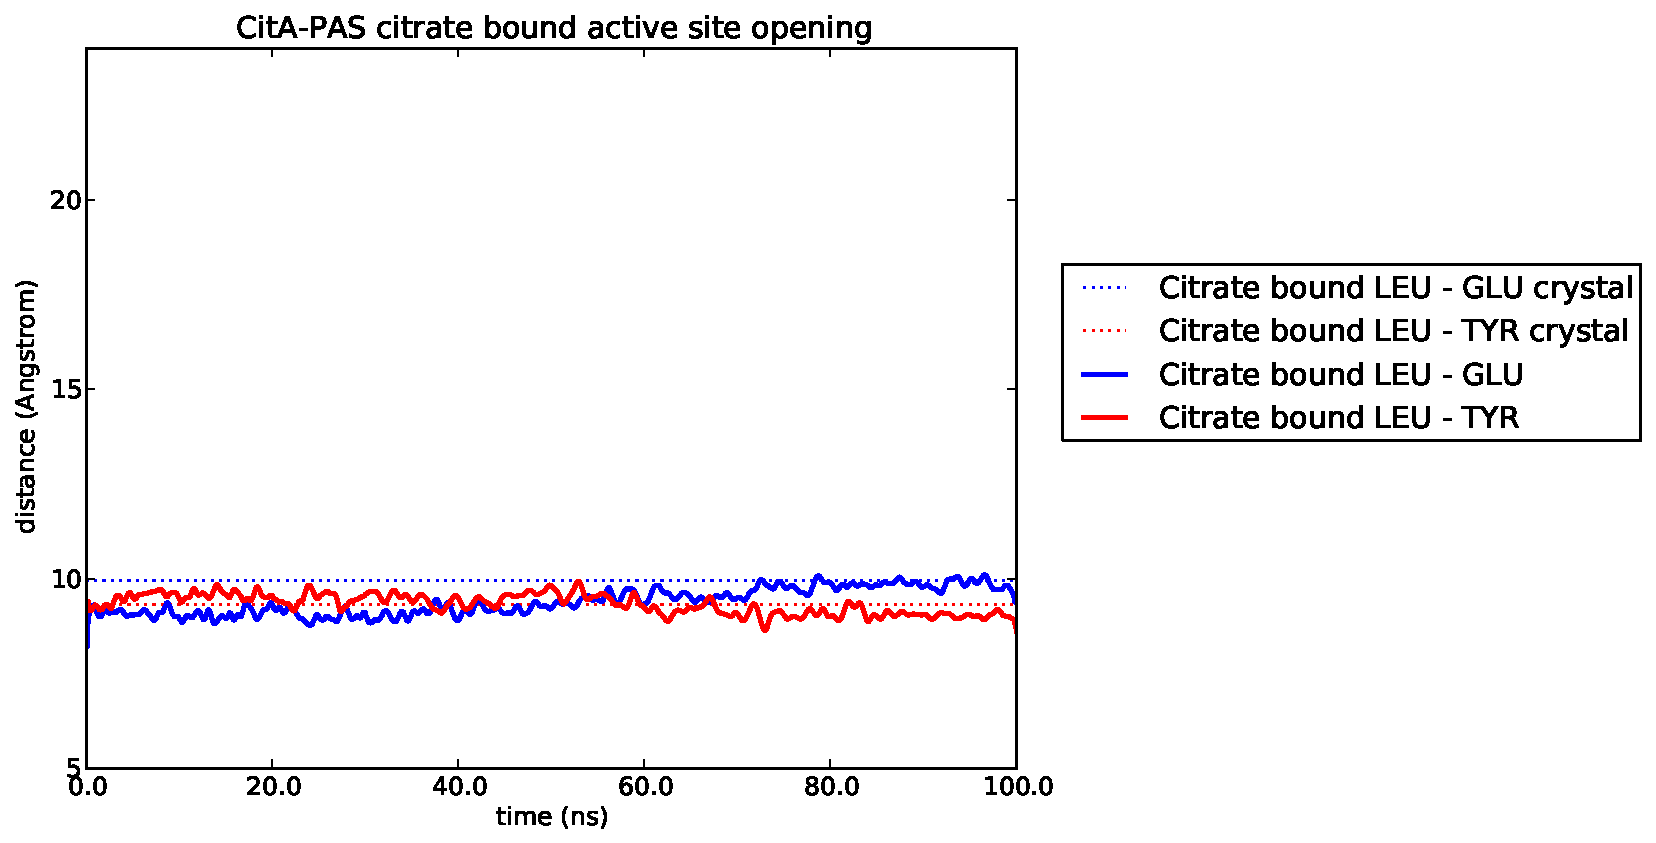
\includegraphics[width=1.0\textwidth]{figures/CitA_opening_citrate_bound.pdf}
    \caption{The plot shows the distances defined in Figure \ref{fig:CitA_pocket} (same color coding) during 100ns MD trajectories. The respective distances in the crystal structures are drawn with a dashed line. The top panel corresponds to the citrate free, the bottom panel to the citrate bound case.}
    \label{fig:CitA_opening_distances}
\end{figure}       



\subsection{Uncomplexed BSLA MD}

\begin{figure}
    \begin{minipage}[]{0.45\linewidth}
        \centering
        a)
        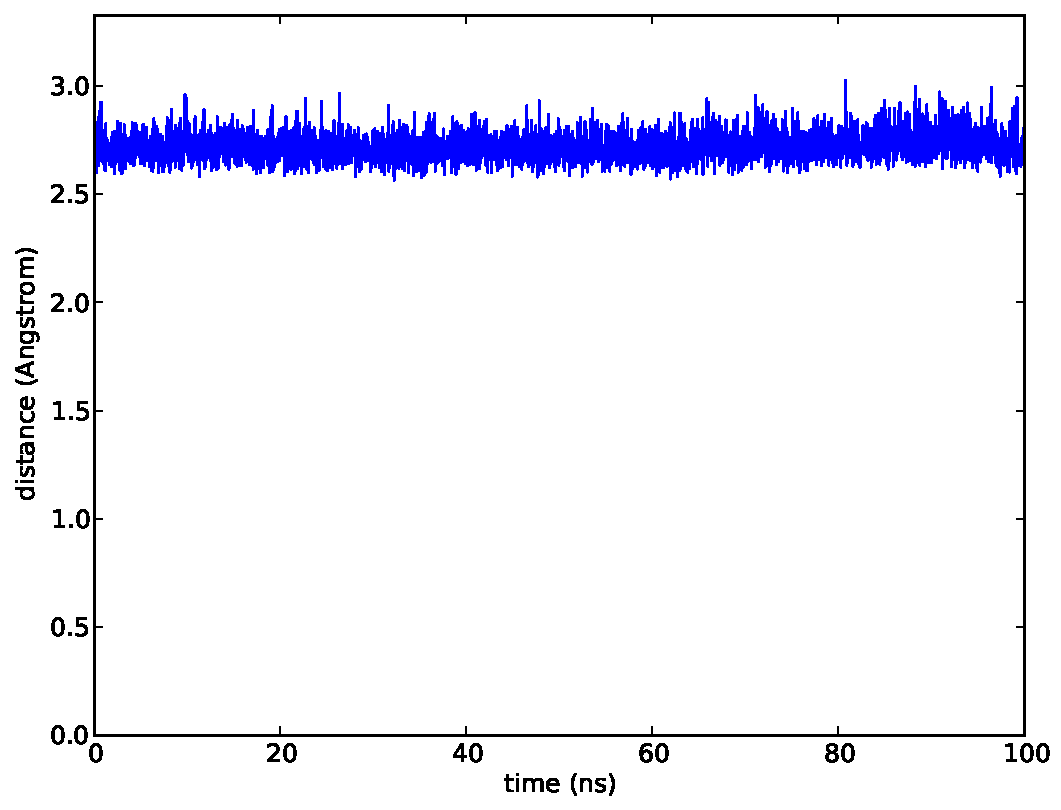
\includegraphics[width=\textwidth]{figures/BSLA_solo/BSLA_solo_dist_ASP133_HIS156.pdf} 
        b)
        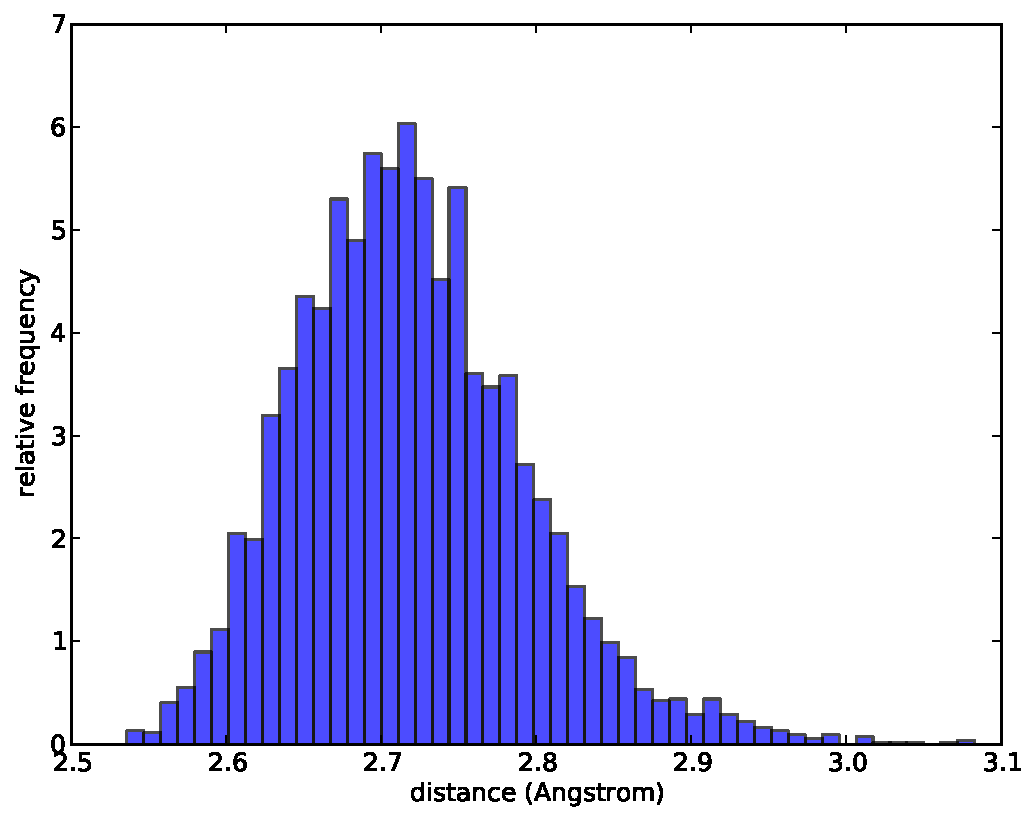
\includegraphics[width=\textwidth]{figures/BSLA_solo/BSLA_distribution_ASP133_HIS156.pdf} 
    \end{minipage}
\hspace{0.5cm}
    \begin{minipage}[]{0.45\linewidth}
        \centering
        c)
        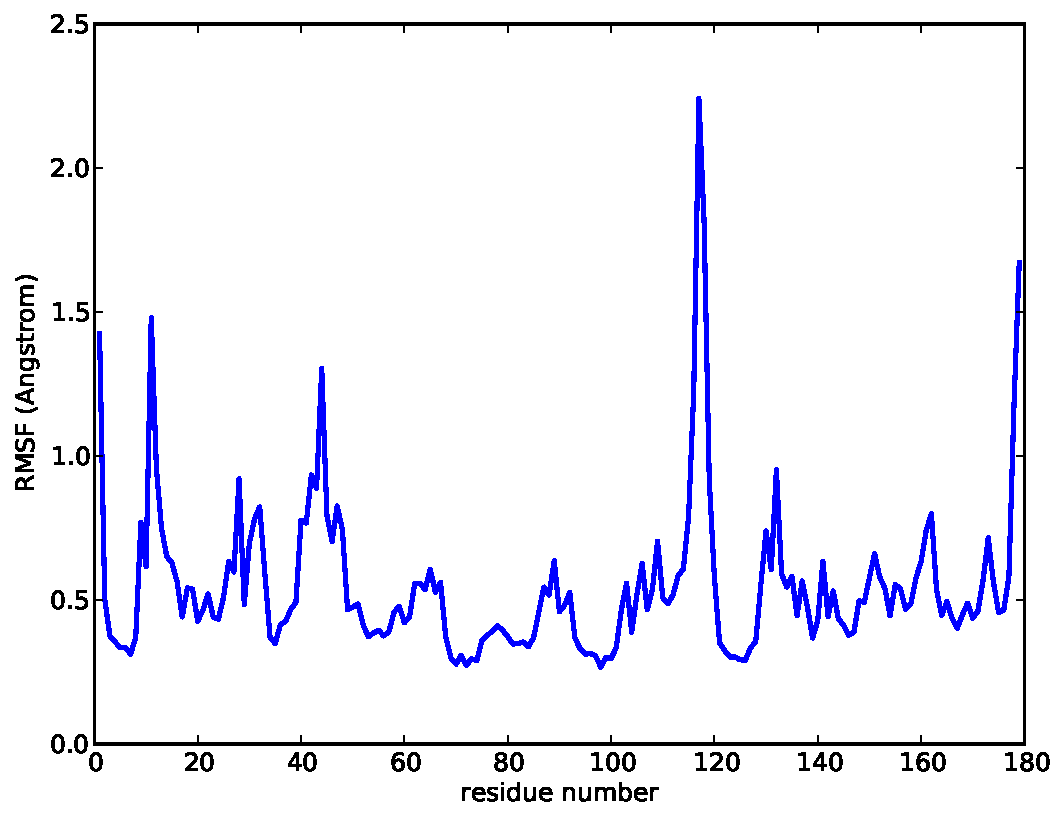
\includegraphics[width=\textwidth]{figures/BSLA_solo/BSLA_solo_rmsf.pdf} 
    \end{minipage}
    \caption{\textbf{a)} Shortest distance between side chain atoms of BSLA active site residues ASP133 and HIS156 during a 100 ns MD trajectory.
    \textbf{b)} Distribution of the distance from a).
    \textbf{c)} Root mean square fluctuation (RMSF) of C$_\alpha$ atoms around the average structure of the 100 ns MD trajectory.}
\label{fig:BSLA_solo}
\end{figure} 






\subsection{Complex Basin Hopping}

\begin{figure}
    \centering
    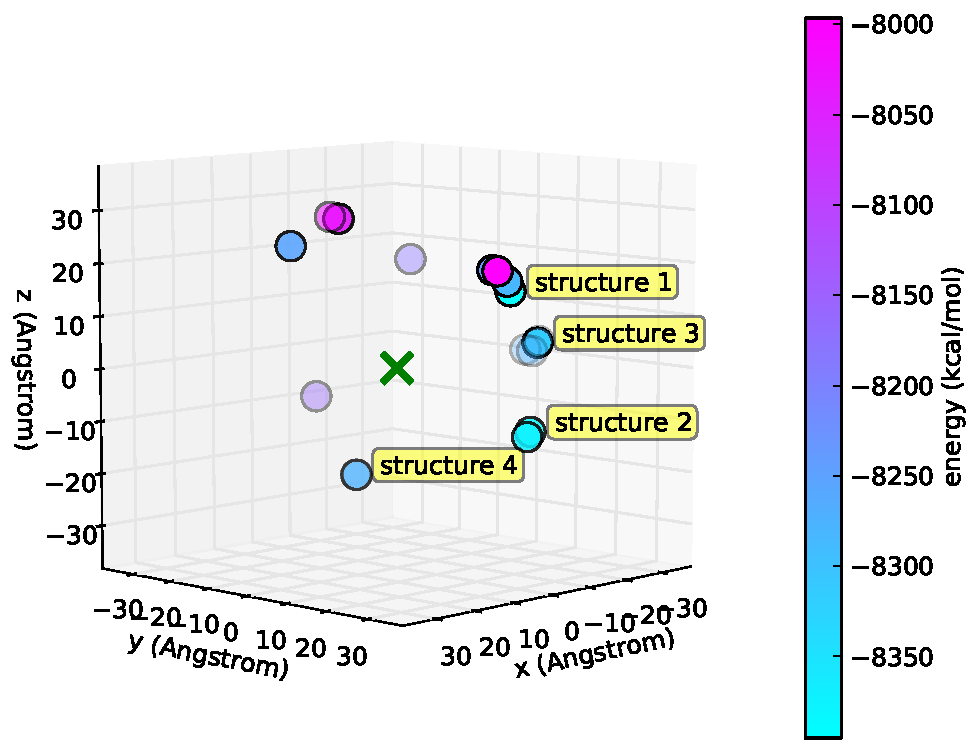
\includegraphics[width=1.0\textwidth]{figures/GMIN/CitA_phi_theta_3D.pdf}
    \caption{Cluster centers of the GMIN output structures. The green cross indicates the center of mass position of the superimposed CitAP domains. The points correspond to the centers of mass of the BSLA domains of each GMIN output structure. Color codes the energy of the structures as indicated by the colorbar and the alpha value is used as a depth cue. The four structures used in subsequent experiments are labeled.}
    \label{fig:GMIN_results}
\end{figure}       

 

\begin{table}
\centering
\begin{tabular}{c c c c c}
    \hline \hline
    Engery     & BH steps & Max. angular step & Convergence Crit. & GMIN run \\ 
    (kcal/mol) &          & size (degree)     & (kcal/mol)        & rank     \\
    \hline
    \rowcolor{lightgray}
    -8395.14   & 10000    &  90               & 0.02              & 1        \\ 
    \rowcolor{lightgray}
    -8381.87   &   500    &  60               & 0.02              & 1        \\
    -8372.59   &   500    &  60               & 0.02              & 2        \\
    \rowcolor{lightgray}
    -8340.34   &   500    &  60               & 0.02              & 6        \\
    -8282.96   &  1000    &  90               & 0.02              & 1        \\
    \rowcolor{lightgray}
    -8275.37   &   500    & 120               & 0.02              & 1        \\
    -8274.22   &   500    & 120               & 0.02              & 2        \\
    -8273.80   &   500    &  30               & 0.02              & 1        \\
    -8273.46   &   500    &  30               & 0.02              & 2        \\
    -8267.76   &   500    &  30               & 0.02              & 7        \\
    -8254.04   &  1000    &  90               & 0.05              & 1        \\
    -8237.37   &   500    &  90               & 0.02              & 1        \\
    -8177.33   &   500    &  90               & 0.02              & 1        \\
    -8156.23   &  1000    &  90               & 0.1               & 1        \\
    -8044.41   &   100    &  90               & 0.02              & 1        \\
    -8038.14   &   100    &  90               & 0.02              & 2        \\
    -8021.09   &   100    &  90               & 0.02              & 9        \\
    -7996.48   &  1000    &  90               & 0.5               & 1        \\
    \hline \hline
\end{tabular}
\caption{Representative structures for the clusters of GMIN output structures ranked according to the lowest energy.
The number of Basin Hopping (BH) steps, the maximum angular step size and the convergence criterium for the energy minimization are given, as well as the rank of each structure in the GMIN run in which they have been obtained.
    The four structures used in subsequent experiemnts are shaded in grey and referenced in the text according to their enumeration as structures 1 to 4.}
\label{tab:GMIN_structures}
\end{table} 



\subsection{CitAP--BSLA fusion protein MD}


% ============================================================================ %

\section{Discussion}

% ============================================================================ %

\section{Conclusion}

% ============================================================================ %



% ============================================================================ %

\pagebreak

\singlespacing
\small

\bibliographystyle{unsrt}
\bibliography{masterthesis}
 
% ============================================================================ %

\end{document}
 
